\begin{exo}
  \donnee{Dans sa tournée, un voyageur de commerce doit se rendre de la ville A à la ville B. Il dispose de deux itinéraires : le premier en passant par la ville C et le second par la ville D. Aucune liaison directe entre A et B existe.  Les temps en heures (h) que passe sur la route le voyageur de commerce pour se déplacer de A à B via les villes C et D peuvent être représentés par des variables aléatoires indépendantes $X_1,X_2,X_3,X_4$ définies par
  \begin{enumerate}
  	\item $X_1$ : "Durée du trajet entre les villes A et C";
  	\item $X_2$ : "Durée du trajet entre les villes C et B";
  	\item $X_3$ : "Durée du trajet entre les villes A et D";
  	\item $X_4$ : "Durée du trajet entre les villes D et B";
  \end{enumerate}
On suppose que ces variables aléatoires sont toutes issues d'une distribution normale. Les temps espérés pour se déplacer d'une ville à l'autre se trouvent dans la figure ci-dessous et le coefficient de variation de chacune de ces variables aléatoires vaut 0.2.
\begin{center}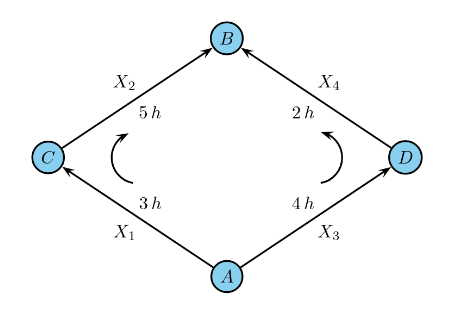
\includegraphics[scale=0.8]{ex5}\end{center}
}
	\begin{subexo}{Le coefficient de variation $\delta_X$ d'une variable aléatoire X est donné par $\frac{\sigma_X}{\mu_X}$. Calculer les écarts-type des variables $X_1,X_2,X_3,X_4$.}
	\end{subexo}	
	\begin{subexo}{Calculer la probabilité que le trajet entre la ville A et B via C dure moins de 9 heures.}
	\end{subexo}
	\begin{subexo}{Déterminer la probabilité que la durée du trajet entre A et B via C soit plus courte que celle via D en considérant la varible aléatoire $T = T_1 - T_2$ ou $T_1$ représente la durée du trajet via C et $T_2$ celle du trajet via D.}
	\end{subexo}
\end{exo}
